‫
‫‫\section*{بخش تشریحی}
‫‫‫\section{سوال اول}
‫
‫الف) شمای ستاره‌ای در زمینهٔ ذخیره و سازماندهی داده‌ها به منظور تجزیه و تحلیل و گزارش‌دهی استفاده می‌شود. مزیت اصلی استفاده از شمای ستاره‌ای آسانی  تجزیه و تحلیل داده‌هاست. در شمای ستاره‌ای، داده‌ها به دو دسته‌ی اصلی تقسیم می‌شوند: \newline
‫۱) \LR{Fact table}: این جدول حاوی اطلاعات اصلی است. \newline
‫۲) \LR{Dimension tables}: این جداول حاوی اطلاعات توصیفی در مورد ابعاد مختلف داده‌های موجود در \LR{Fact table} هستند. \newline
‫با توجه به ساختار اصلی شمای‌ ستاره‌ای، برای ذخیره‌ی اطلاعات پروازهای خارجی این شما به شکل زیر می‌باشد.
‫
‫\begin{center}
‫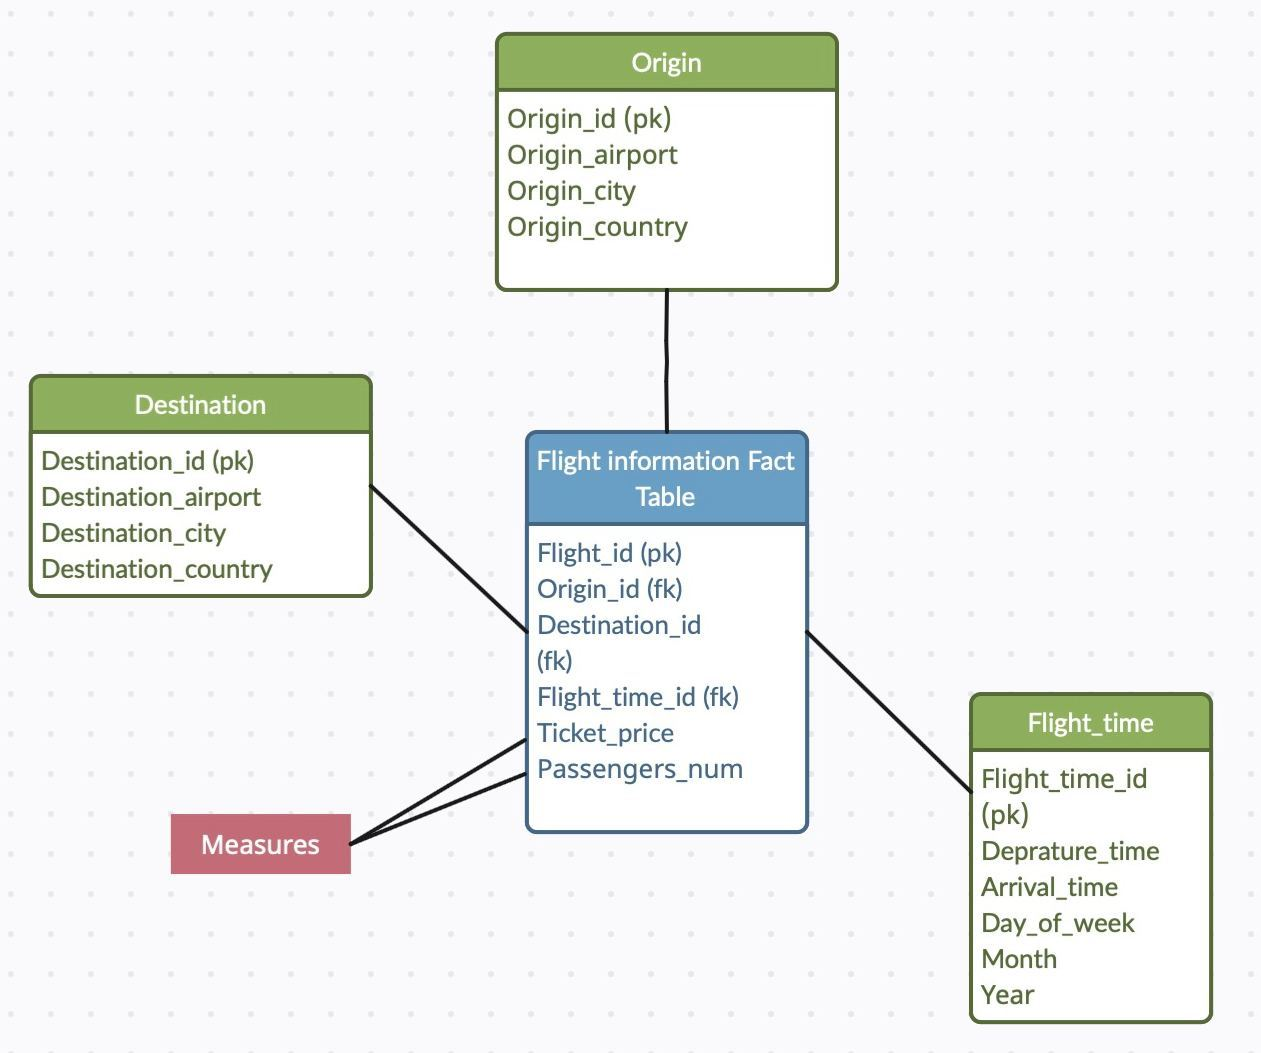
\includegraphics[scale=0.35]{figs/star_schema1.png}
‫\end{center}
‫
‫ویژگی‌های (attributes) هر کدام از بعدها در \LR{Dimension tables} خود آورده شده است. همچنین لازم به ذکر است که \LR{Flight-id} در \LR{Fact table} به عنوان کلید اصلی در نظر گرفته شده است. بسته به نیازی که تصور می‌شود می توان آن را حذف کرد یا نگه داشت. اما به صورت کلی وجود یک متغیر منحصر به فرد برای ثبت و پرس و جوی داده‌ها مناسب است.
‫\vspace{1cm}
‫
‫ب)  برای این مقایسه هر کدام از میانگین‌ها محاسبه و در پایان با یکدیگر مقایسه شده است. \newline
‫میانگین قیمت بلیط‌های تهران به میلان در خرداد ماه سال ۱۴۰۲: \newline
‫
\LR{\LR{Roll up on origin (from Origin-airport to Origin-city)} \newline
\LR{Roll up on Destination (from Destination-airport to Destination-city)} \newline
\LR{Roll up on Flight-time (from Departure-time to Month)} \newline
\LR{Dice for (Origin = “Tehran”) and (Destination = “Milan”)} \newline
\LR{Dice for (Flight-time = “Khordad”)} \newline
\LR{Roll up on Flight-time (from Month to Year)} \newline
\LR{Dice for (Flight-time = 1402(} \newline
\LR{Select AVG(Ticket-price)} \newline}

‫‫میانگین قیمت بلیط‌های تهران به آمستردام در فروردین ماه سال ۱۴۰۱: \newline
‫
\LR{\LR{Roll up on origin (from Origin-airport to Origin-city)} \newline
\LR{Roll up on Destination (from Destination-airport to Destination-city)} \newline
\LR{Roll up on Flight-time (from Departure-time to Month)} \newline
\LR{Dice for (Origin = “Tehran”) and (Destination = “Amesterdam”)} \newline
\LR{Dice for (Flight-time = “Farvardin”)} \newline
\LR{Roll up on Flight-time (from Month to Year)} \newline
\LR{Dice for (Flight-time = 1401(} \newline
\LR{Select AVG(Ticket-price)} \newline}
‫
‫\vspace{1cm}
‫
‫\hrule height .4 pt depth 0 pt width 16 cm \relax
‫
‫%------------------------------------------------------------------
‫
‫‫\section{سوال دوم}
‫
‫الف)‌ برای پیمایش بهینه در chunk ها باید توجه داشت که صفحات بر اساس اندازه‌شان به ترتیب صعودی محاسبه می‌شوند. در این سوال صفحات ایجاد شده AB , AC و BC هستند که از نظر اندازه‌ی صفحه‌ها به شکل زیر می‌باشند.
‫
\begin{center}
\LR{AC < AB < BC}
\end{center}

‫با توجه به آن که BC کوچک‌تر از بقیه‌ی صفحات می‌باشد بنابراین پیمایش از این صفحه آغاز می‌شود و در ادامه در ستون بعدی در بعد A مجددا محاسبه خواهد شد.
‫
‫‫\vspace{1cm}
‫
‫ب) برای محاسبه‌ی کمترین فضایی که در حافظه‌ی اصلی نیاز است از بهینه‌ترین پیمایش در قسمت الف استفاده می‌شود. ابتدا تعداد معیارها محاسبه می‌شود. برای محاسبه‌ی تعداد آن‌ها، می‌بایست تعداد تمام cell های صفحه‌ی BC در کنار یک chunk از صفحه‌ی AC و یک ستون از صفحه‌ی AB انتخاب شود.
‫

\LR{memory = 4 * )100 * 1000 + 100 * 100000 + 100 * 100000( = 80400000  byte}

‫\vspace{1cm}
‫
‫ج) بهترین روش برای محاسبه‌ی cuboid های یک بعدی با استفاده از cuboid های دو بعدی مانند روش قبل است به این صورت که کوچکترین cuboid های دو بعدی انتخاب می‌شوند (آن‌هایی که تعداد cell کمتری دارند). به همین منظور برای cuboid های یک بعدی A , B و C بهترین حالت استفاده از cuboid های دو بعدی AB , BC و BC است.
‫
‫
‫\vspace{1cm}
‫
‫\hrule height .4 pt depth 0 pt width 16 cm \relax
‫
‫%------------------------------------------------------------------
‫
‫\section{سوال سوم}
‫
‫   الف) با توجه به آن که cuboid های پایه‌ی a داده شده است، بعد i م می‌تواند $a_{i}$ یا $b_i$ باشد. در این حالت تعداد cuboid ها برابر با \colorbox{Emerald}{\(2^9\)} می‌باشد.
‫
‫\vspace{1cm}
‫
‫ب) سلول‌های پایه‌ی غیر تهی aggregate با تعویض a یا b با * ایجاد می‌شوند. با توجه به سلول اول و دوم برای هر کدام \(2^9\) سلول پایه‌ی غیر تهی وجود دارد. اما ۲ تا از این سلول‌ها غیر تهی می‌باشند بنابراین تعداد سلول‌های aggregate غیر تهی برابر با مقدار زیر می‌باشد.
‫\begin{center}
‫\colorbox{Emerald}{تعداد سلول‌های aggregate غیر تهی =2 - \(2^9\)}
‫\end{center}
‫
‫‫\vspace{1cm}
‫
‫ج) تعداد سلول‌های بسته‌ی غیر تهی یک data cube شامل سلول‌های cuboid پایه به علاوه‌ی سلولی که داده‌ها یا مقادیر درون آن، برای تمامی ابعاد مربوطه موجود هستند.‌ در واقع برای این سوال سلول‌های بسته‌ی غیر تهی عبارتند از:
‫
\LR{
\LR{) $a_{1}$, $a_{2}$, $b_{3}$, $a_{4}$, $a_{5}$, $b_{6}$, $a_{7}$, $a_{8}$, $b_{9}$ ( : 15} \newline
\LR{) $b_{1}$, $a_{2}$, $a_{3}$, $b_{4}$, $a_{5}$, $a_{6}$, $b_{7}$, $a_{8}$, $a_{9}$ ( : 10} \newline
\LR{) * , $a_{2}$ , * , * , $a_{5}$ , * , * , $a_{8}$, * ( : 25} \newline
}

‫
‫بنابراین با توجه به سلول‌های ارائه شده تعداد سلول‌های بسته‌ی غیر تهی برابر با \colorbox{Emerald}{3} می‌باشد.
‫
‫‫‫\vspace{1cm}
‫
‫د) با توجه به شرط \LR{minimum support = 20} در این سوال تنها سلول زیر می‌تواند این شرط را ارضا کند. 
\begin{center}
\LR{\LR{) * , $a_{2}$ , * , * , $a_{5}$ , * , * , $a_{8}$, * ( : 25}} 
\end{center}
‫که با توجه به تعداد مقادیر ثابت که می‌توانند یا خودشان باشند یا * باشند تعداد سلول‌های aggregate غیر تهی با شرط \LR{minimum support = 20} برابر با \colorbox{Emerald}{\(2^3\)} می‌باشد.
‫
‫‫\vspace{1cm}
‫
‫\hrule height .4 pt depth 0 pt width 16 cm \relax
‫
‫‫%------------------------------------------------------------------

‫\section{سوال چهارم}

‫الف) بهترین کارایی برای الگوریتم BUC زمانی است که از dimension با cardinality بالاتر پردازش شروع شود. این روش منجر به محاسبات کارآمد با استفاده از pruning بیشتر، تشخیص سریع‌تر سلول‌‌های خالی و کاهش مقدار مموری مصرف می‌باشد. \newline
‫با توجه به روش ارائه شده، پردازش در این سوال از occupation شروع شده، با education ادامه می‌یابد و در نهایت پردازش با بعد Gender به پایان می‌رسد. زیرا تعداد مقادیر متمایز در occupation برابر با ۴ ، در education برابر با ۳ و در Gender مقادیر متمایز برابر با ۲ می‌باشد.

‫\vspace{1cm}
‫
‫ب) با توجه به تعریف بهترین روش برای الگوریتم BUC ، درخت پردازش برای این سوال رسم شده است. درخت پردازش به این نحو عمل می‌کند که اگر شرط \LR{ minimum support = 3} برای یک شاخه ارضا شود به زیرشاخه‌های دیگر نفوذ می‌کند در غیر این صورت از آن شاخه می‌گذرد و آن شاخه در درخت پردازش لحاظ نمی‌شود. شکل زیر این درخت را نشان می‌دهد. 
‫
‫\begin{center}
‫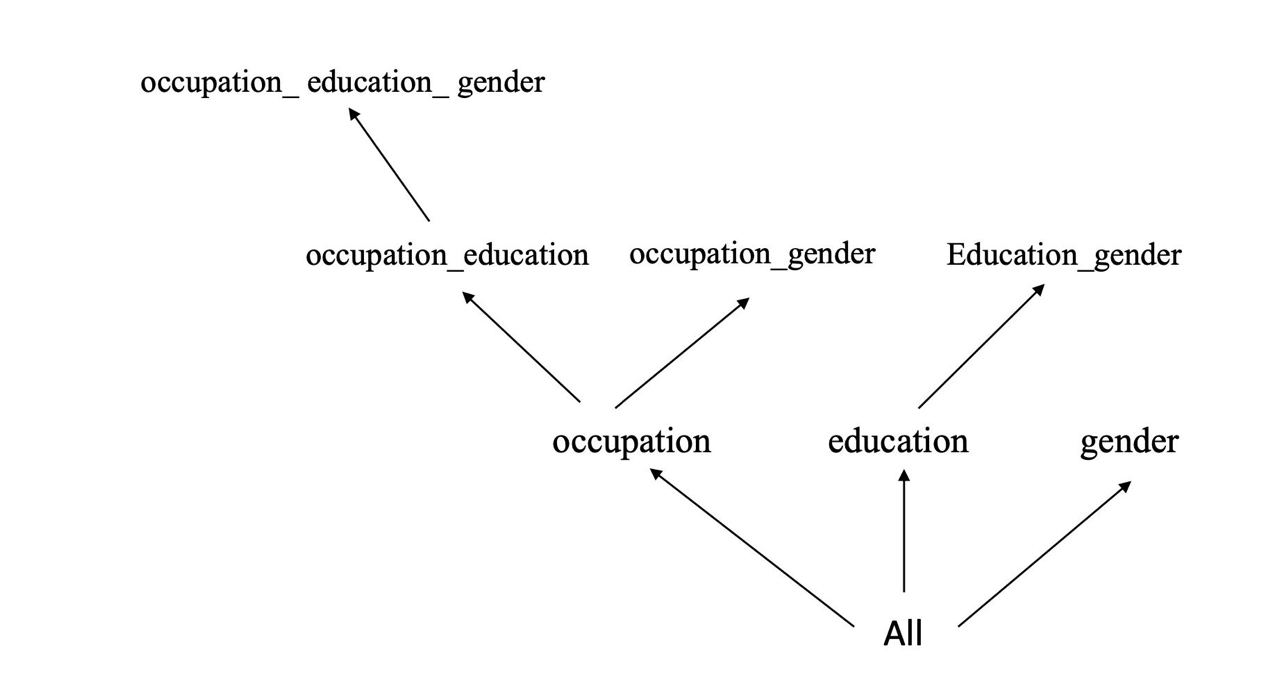
\includegraphics[scale=0.35]{figs/tree.png}
‫\end{center}
‫
‫در \LR{Iceberg cube} شرط \LR{minimum support = 3} برقرار است که به معنای آن است که یک cube باید حداقل ۳ عضو داشته باشد. با توجه به درخت رسم شده، پردازش از اول درخت، یعنی All شروع می‌شود. cube متناظر با این سطح ( * ، * ، * ) می‌باشد که همه‌ی تعداد مقادیر را شامل می‌شود و تعداد آن ۱۰ تا می‌باشد. سپس این الگوریتم به سراغ occupation می‌رود و شرط \LR{minimum support = 3} را برای همه‌ی مقادیر این بعد بررسی می‌کند. نتیجه در زیر آورده شده است.
‫
\LR{
\LR{) programmer ، * ، * ( : 4}  \colorbox{YellowGreen}{not prune} \newline
\LR{) teacher ، * ، * ( : 3}  \colorbox{YellowGreen}{not prune} \newline
\LR{) CEO ، * ، * ( : 2}  \colorbox{red}{prune}\newline
\LR{) doctor ، * ، * ( : 1}  \colorbox{red}{prune} \newline
}
‫
‫با توجه به مقادیر فوق ( * , * , CEO ) و ( * , * , teacher ) حذف یا prune می‌شوند. \newline
‫این الگوریتم در ادامه برای هر کدام از cube های prune نشده مقادیر موجود را بررسی می‌‌کند. با توجه به ترتیب انتخاب شده در بخش اول، بعد education بعد از بعد occupation قرار می‌گیرد. \newline
‫
\LR{
\LR{) programmer ، college ، * ( : 3}  \colorbox{YellowGreen}{not prune} \newline
\LR{) teacher ، college ، * ( : 2}  \colorbox{red}{prune} \newline
\LR{) programmer ، high school ، * ( : 1}  \colorbox{red}{prune}\newline
\LR{) teacher ، graduate ، * ( : 1}  \colorbox{red}{prune} \newline
}
‫با توجه به آن که ( * , programmer , college ) شرط را ارضا کرد و prune نشد همچنان این الگوربتم برای بعد gender نیز شرط را بررسی می‌کند. 
‫
\LR{
\LR{) programmer ، college ، female ( : 2}  \colorbox{red}{prune}\newline
\LR{) programmer ، high school ، male ( : 1}  \colorbox{red}{prune}\newline
}

‫با توجه به نتیجه‌ی حاصل الگوریتم در این نقطه از شاخه‌ی مربوط به occupation-education-gender خارج شده و وارد occupation-gender می‌شود تا شرط \LR{Iceberg cube} را بررسی کند. نتیجه به شکل زیر خواهد بود.
‫
\LR{
\LR{) programmer ، * ، female ( : 2}  \colorbox{red}{prune} \newline
\LR{) teacher ، * ، male ( : 2}  \colorbox{red}{prune} \newline
\LR{) teacher ، * ، female ( : 1}  \colorbox{red}{prune}\newline
\LR{) teacher ، * ، male ( : 1}  \colorbox{red}{prune} \newline
}
‫با توجه به prune شدن تمام cube ها و عدم وجود حالت دیگر در شاخه‌ی occupation این الگوریتم از این شاخه خارج می‌شود و وارد شاخه‌ی education می‌شود. نتیجه در زیر آورده شده است. 
‫
\LR{
\LR{) * ، college ، * ( : 5}  \colorbox{YellowGreen}{not prune} \newline
\LR{) * ، high school ، * ( : 3}  \colorbox{YellowGreen}{not prune} \newline
\LR{) * ، graduate ، * ( : 2}  \colorbox{red}{prune}\newline
}
‫از آنجایی که ترکیب بعد occupation با education بررسی شده است در ادامه این شاخه بعد gender بررسی می‌شود. نتیجه به شکل زیر خواهد بود.
‫
\LR{
\LR{) * ، college ، female ( : 3}  \colorbox{YellowGreen}{not prune} \newline
\LR{) * ، college ، male ( : 2}  \colorbox{red}{prune} \newline
\LR{) * ، high school ، male ( : 2}  \colorbox{red}{prune}\newline
\LR{) * ، high school ، female ( : 1}  \colorbox{red}{prune}\newline
}
‫
‫از آن جایی که در قسمت قبل occupation-education-gender بررسی شده است الگوریتم وارد شاخه‌ی اصلی gender می‌شود. نتیجه‌ی بررسی این شرط در زیر آورده شده است. 
‫
\LR{
\LR{) * ، * ، female ( : 5}  \colorbox{YellowGreen}{not prune} \newline
\LR{) * ، * ، male ( : 5}  \colorbox{YellowGreen}{not prune} \newline
}

‫در نتیجه \LR{Iceberg cube} با شرط \LR{minimum support = 3} به شکل زیر می‌باشد.
‫
\LR{
\LR{) * ، * ، * ( : 10} \newline
\LR{) * ، * ، female ( : 5} \newline
\LR{) * ، * ، male ( : 5} \newline
\LR{) * ، college ، * ( : 5} \newline
\LR{) programmer ، * ، * ( : 4} \newline
\LR{) teacher ، * ، * ( : 3} \newline
\LR{) programmer ، college ، * ( : 3} \newline
\LR{) * ، high school ، * ( : 3} \newline
\LR{) * ، college ، female ( : 3} \newline
}

‫‫\vspace{1cm}
‫
‫\hrule height .4 pt depth 0 pt width 16 cm \relax
‫
‫‫%------------------------------------------------------------------
‫
‫‫‫\section*{بخش عملی}
‫
‫